\documentclass{article}
\usepackage[paperwidth=32cm,paperheight=18cm,margin=0.9cm]{geometry}
\usepackage{tikz}
\usetikzlibrary{arrows.meta,positioning}
\usepackage[T1]{fontenc}
\usepackage{helvet}
\renewcommand{\familydefault}{\sfdefault}
\pagestyle{empty}
\definecolor{ink}{HTML}{14202B}
\definecolor{teal}{HTML}{0C5F59}
\definecolor{paper}{HTML}{F4F1EA}
\definecolor{sand}{HTML}{E7DCC8}
\definecolor{brown}{HTML}{5C4A3A}
\definecolor{line}{HTML}{8A8175}

\tikzset{
  card/.style={draw=ink, line width=1pt, rounded corners=4pt, align=center, inner sep=10pt, fill=white, font=\large},
  bar/.style={card, text=white, minimum height=1.7cm},
  small/.style={font=\normalsize},
  every picture/.style={line width=1.1pt}
}

\begin{document}
\pagecolor{paper}
\begin{center}
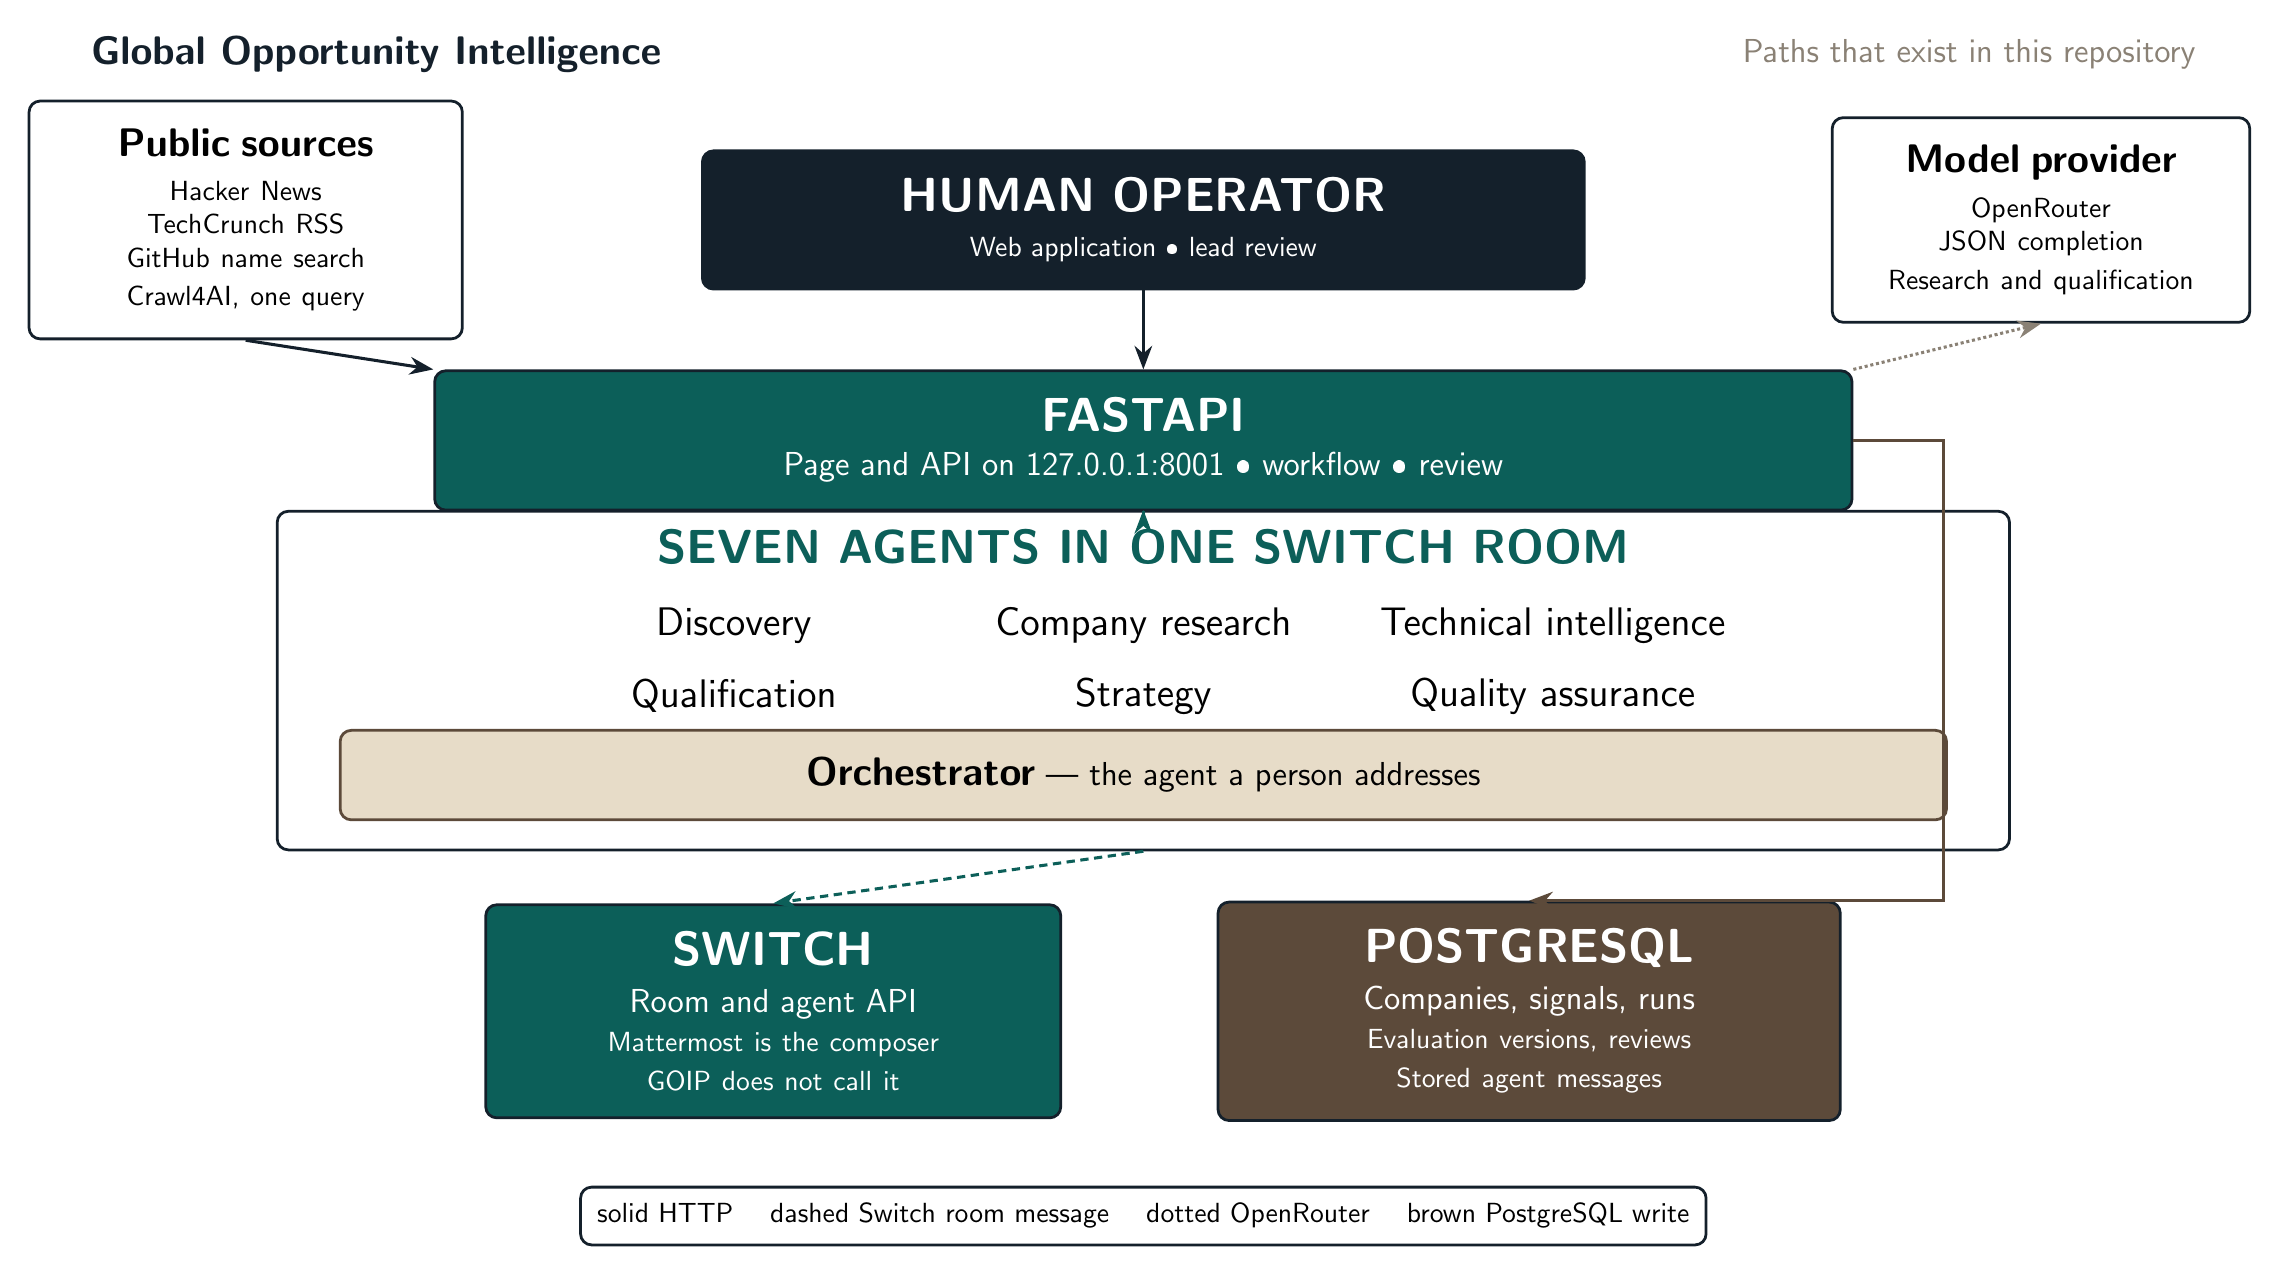
\begin{tikzpicture}
  \node[font=\Large\bfseries, text=ink, anchor=west] at (-13.5,7.6) {Global Opportunity Intelligence};
  \node[font=\large, text=line, anchor=east] at (13.5,7.6) {Paths that exist in this repository};

  \node[card, text width=4.8cm] (sources) at (-11.4,5.5) {
    {\Large\bfseries Public sources}\\[4pt]
    {\normalsize Hacker News\\ TechCrunch RSS\\ GitHub name search\\ Crawl4AI, one query}
  };
  \node[card, text width=4.6cm] (model) at (11.4,5.5) {
    {\Large\bfseries Model provider}\\[4pt]
    {\normalsize OpenRouter\\ JSON completion\\ Research and qualification}
  };

  \node[bar, fill=ink, minimum width=11.2cm] (human) at (0,5.5) {{\LARGE\bfseries HUMAN OPERATOR}\\[2pt]{\normalsize Web application \textbullet\ lead review}};
  \node[bar, fill=teal, minimum width=18cm] (api) at (0,2.7) {{\LARGE\bfseries FASTAPI}\\[2pt]{\large Page and API on 127.0.0.1:8001 \textbullet\ workflow \textbullet\ review}};

  \node[card, minimum width=22cm, minimum height=4.3cm, fill=white] (agents) at (0,-0.35) {};
  \node[font=\LARGE\bfseries, text=teal] at (0,1.35) {SEVEN AGENTS IN ONE SWITCH ROOM};
  \node[font=\Large] at (-5.2,0.35) {Discovery};
  \node[font=\Large] at (0,0.35) {Company research};
  \node[font=\Large] at (5.2,0.35) {Technical intelligence};
  \node[font=\Large] at (-5.2,-0.55) {Qualification};
  \node[font=\Large] at (0,-0.55) {Strategy};
  \node[font=\Large] at (5.2,-0.55) {Quality assurance};
  \node[card, fill=sand, minimum width=20.4cm, minimum height=1.05cm, draw=brown] at (0,-1.55) {{\Large\bfseries Orchestrator} {\large --- the agent a person addresses}};

  \node[card, fill=teal, text=white, text width=6.6cm, minimum height=2.5cm] (switch) at (-4.7,-4.55) {
    {\LARGE\bfseries SWITCH}\\[3pt]
    {\large Room and agent API}\\
    {\normalsize Mattermost is the composer}\\
    {\normalsize GOIP does not call it}
  };
  \node[card, fill=brown, text=white, text width=7.2cm, minimum height=2.5cm] (db) at (4.9,-4.55) {
    {\LARGE\bfseries POSTGRESQL}\\[3pt]
    {\large Companies, signals, runs}\\
    {\normalsize Evaluation versions, reviews}\\
    {\normalsize Stored agent messages}
  };

  \draw[-{Stealth[length=3mm]}, ink] (human.south) -- (api.north);
  \draw[-{Stealth[length=3mm]}, ink] (sources.south) -- (api.north west);
  \draw[-{Stealth[length=3mm]}, line, densely dotted] (api.north east) -- (model.south);
  \draw[-{Stealth[length=3mm]}, teal, densely dashed] (api.south) -- (agents.north);
  \draw[-{Stealth[length=3mm]}, teal, densely dashed] (agents.south) -- (switch.north);
  \draw[-{Stealth[length=3mm]}, brown] (api.east) -- ++(1.15,0) |- (db.north);

  \node[card, font=\normalsize, inner sep=6pt] at (0,-7.15) {solid HTTP \quad dashed Switch room message \quad dotted OpenRouter \quad brown PostgreSQL write};
\end{tikzpicture}
\end{center}

\newpage
\begin{center}
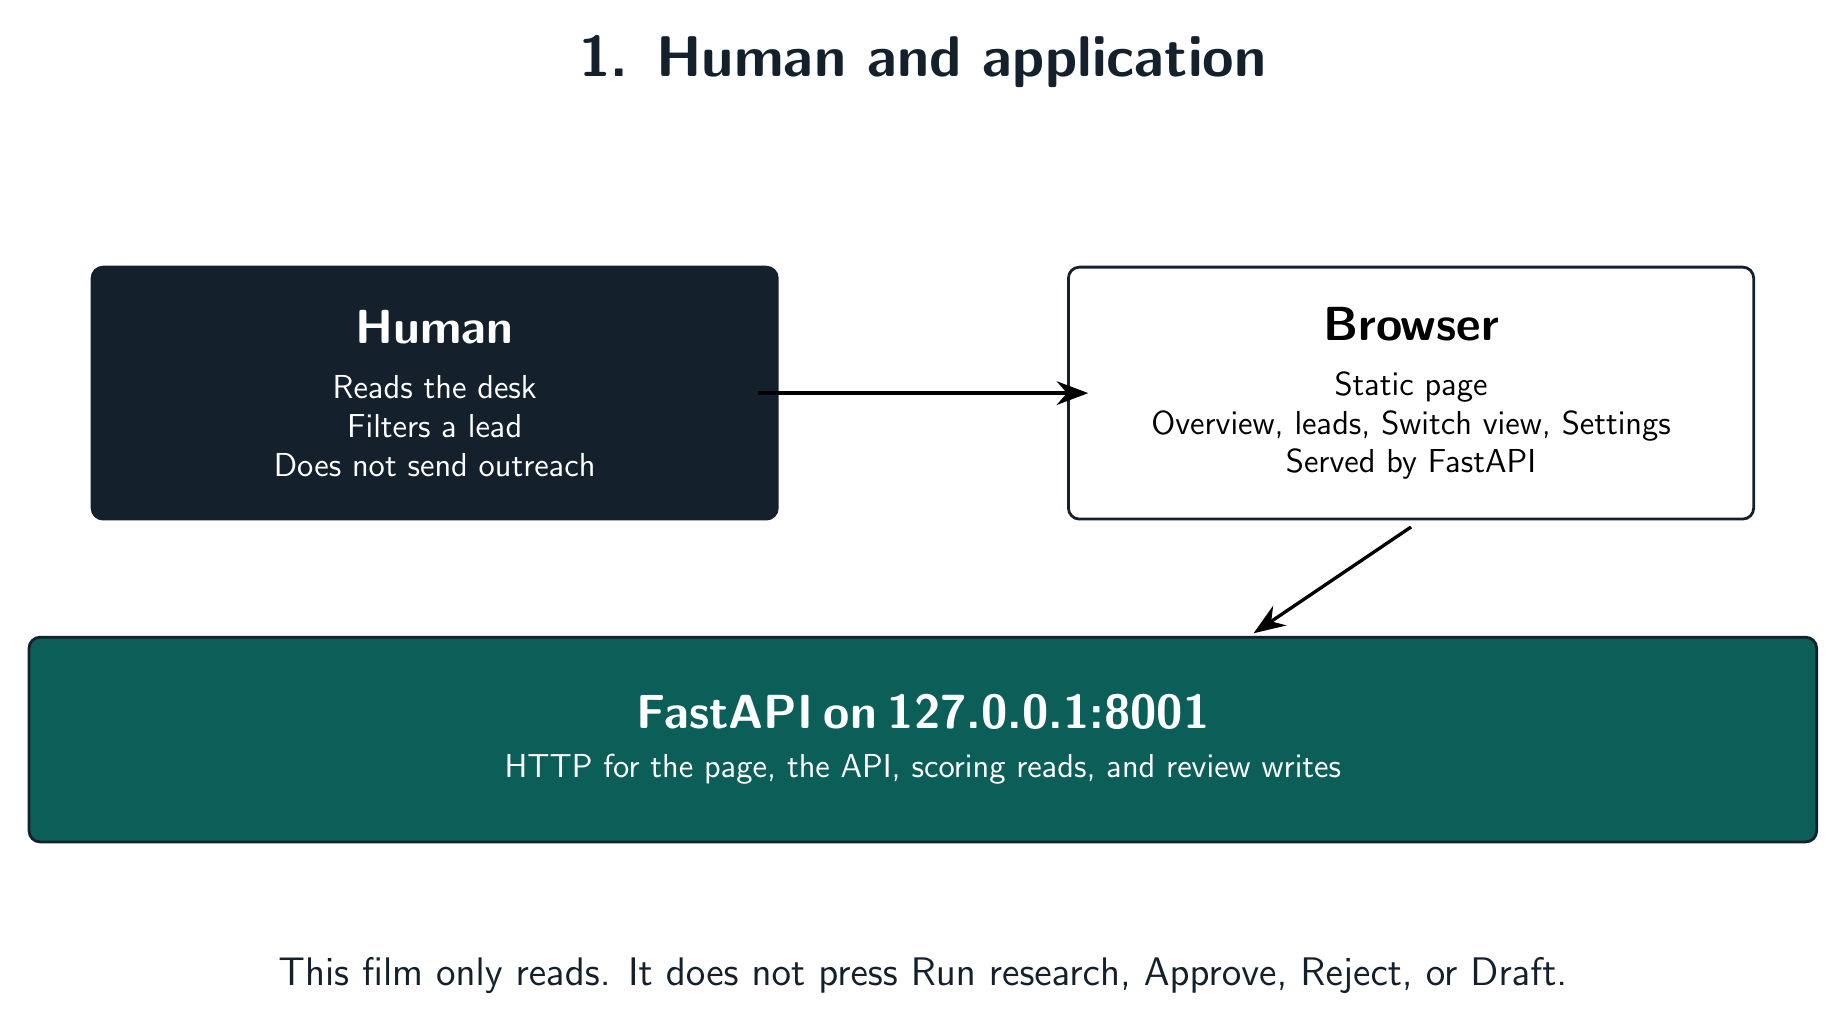
\begin{tikzpicture}
  \node[font=\huge\bfseries, text=ink] at (0,6.4) {1. Human and application};
  \node[card, fill=ink, text=white, text width=8cm, minimum height=3.2cm] at (-6.2,2.2) {{\LARGE\bfseries Human}\\[6pt]\large Reads the desk\\ Filters a lead\\ Does not send outreach};
  \node[card, text width=8cm, minimum height=3.2cm] at (6.2,2.2) {{\LARGE\bfseries Browser}\\[6pt]\large Static page\\ Overview, leads, Switch view, Settings\\ Served by FastAPI};
  \node[card, fill=teal, text=white, text width=22cm, minimum height=2.6cm] at (0,-2.2) {{\LARGE\bfseries FastAPI on 127.0.0.1:8001}\\[4pt]\large HTTP for the page, the API, scoring reads, and review writes};
  \node[font=\Large, text=ink, align=center] at (0,-5.2) {This film only reads. It does not press Run research, Approve, Reject, or Draft.};
  \draw[-{Stealth[length=4mm]}, very thick] (-2.1,2.2) -- (2.1,2.2);
  \draw[-{Stealth[length=4mm]}, very thick] (6.2,0.5) -- (4.2,-0.85);
\end{tikzpicture}
\end{center}

\newpage
\begin{center}
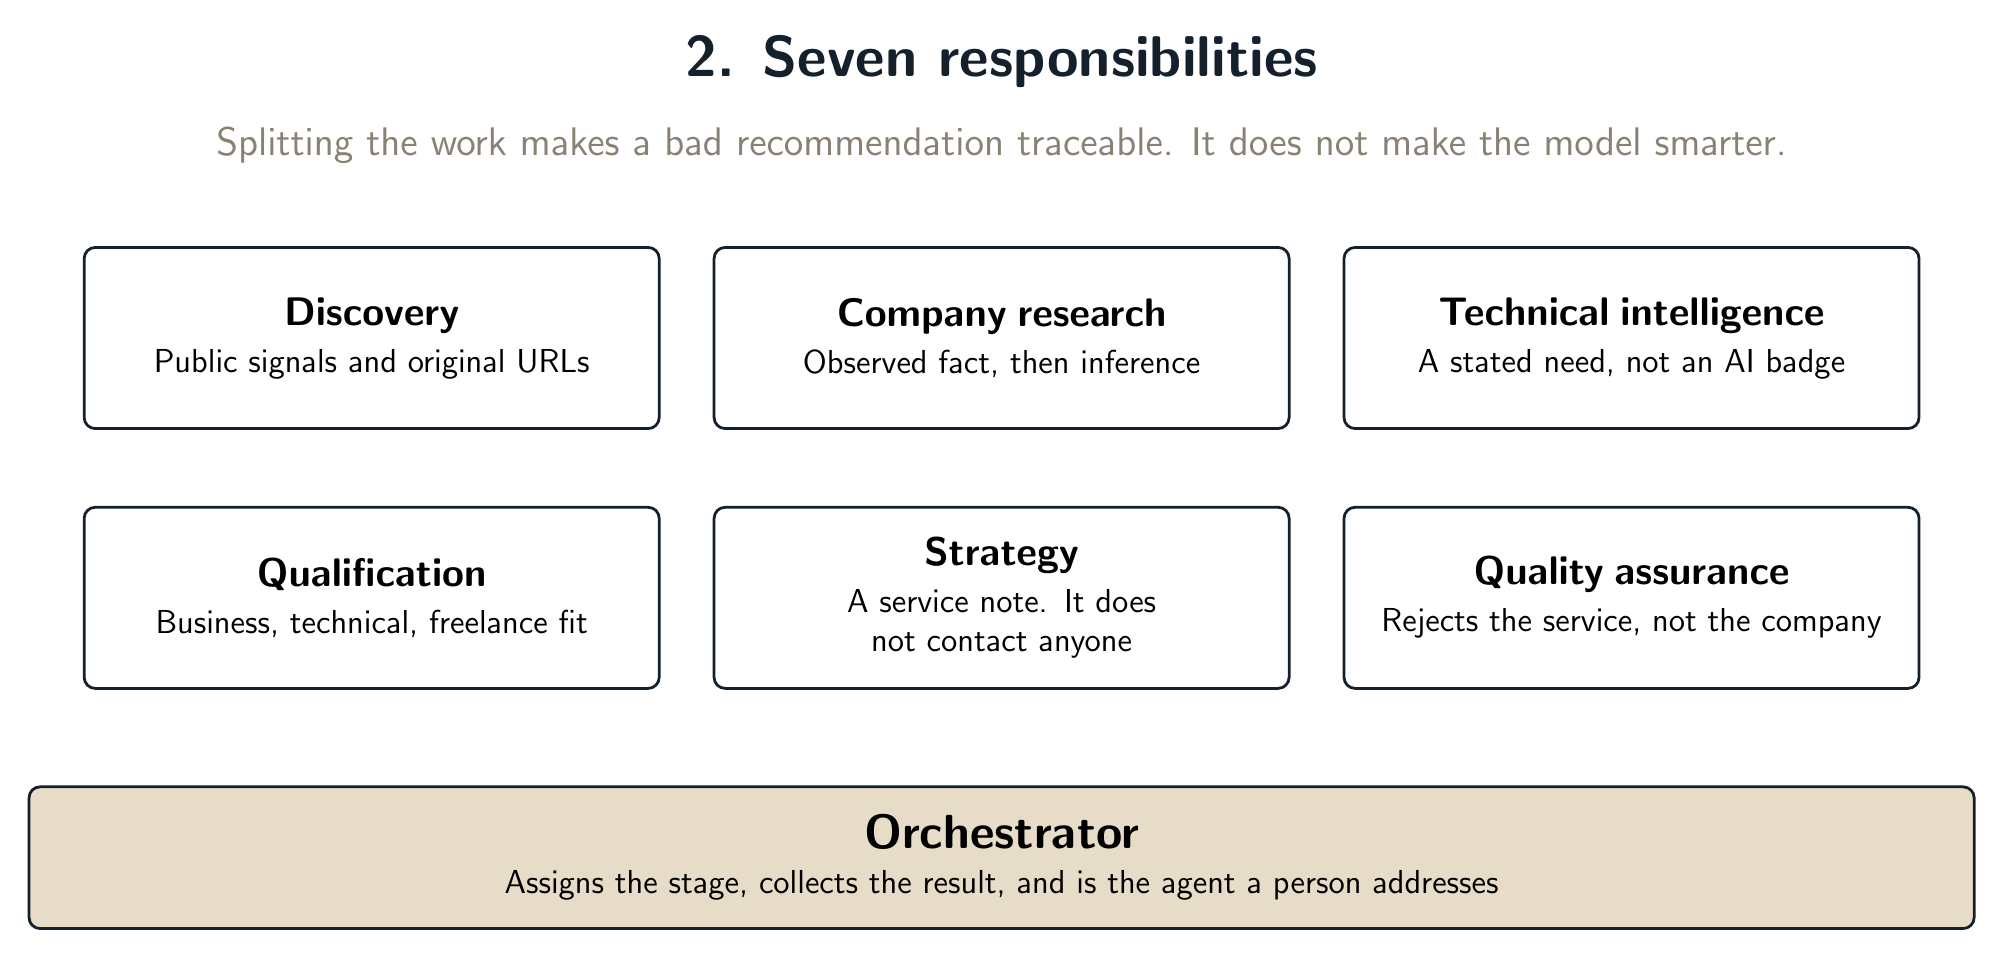
\begin{tikzpicture}
  \node[font=\huge\bfseries, text=ink] at (0,6.6) {2. Seven responsibilities};
  \node[font=\Large, text=line] at (0,5.55) {Splitting the work makes a bad recommendation traceable. It does not make the model smarter.};
  \node[card, text width=6.6cm, minimum height=2.3cm] at (-8,3.1) {{\Large\bfseries Discovery}\\[3pt] Public signals and original URLs};
  \node[card, text width=6.6cm, minimum height=2.3cm] at (0,3.1) {{\Large\bfseries Company research}\\[3pt] Observed fact, then inference};
  \node[card, text width=6.6cm, minimum height=2.3cm] at (8,3.1) {{\Large\bfseries Technical intelligence}\\[3pt] A stated need, not an AI badge};
  \node[card, text width=6.6cm, minimum height=2.3cm] at (-8,-0.2) {{\Large\bfseries Qualification}\\[3pt] Business, technical, freelance fit};
  \node[card, text width=6.6cm, minimum height=2.3cm] at (0,-0.2) {{\Large\bfseries Strategy}\\[3pt] A service note. It does not contact anyone};
  \node[card, text width=6.6cm, minimum height=2.3cm] at (8,-0.2) {{\Large\bfseries Quality assurance}\\[3pt] Rejects the service, not the company};
  \node[card, fill=sand, text width=24cm, minimum height=1.8cm] at (0,-3.5) {{\LARGE\bfseries Orchestrator}\\[2pt]\large Assigns the stage, collects the result, and is the agent a person addresses};
\end{tikzpicture}
\end{center}

\newpage
\begin{center}
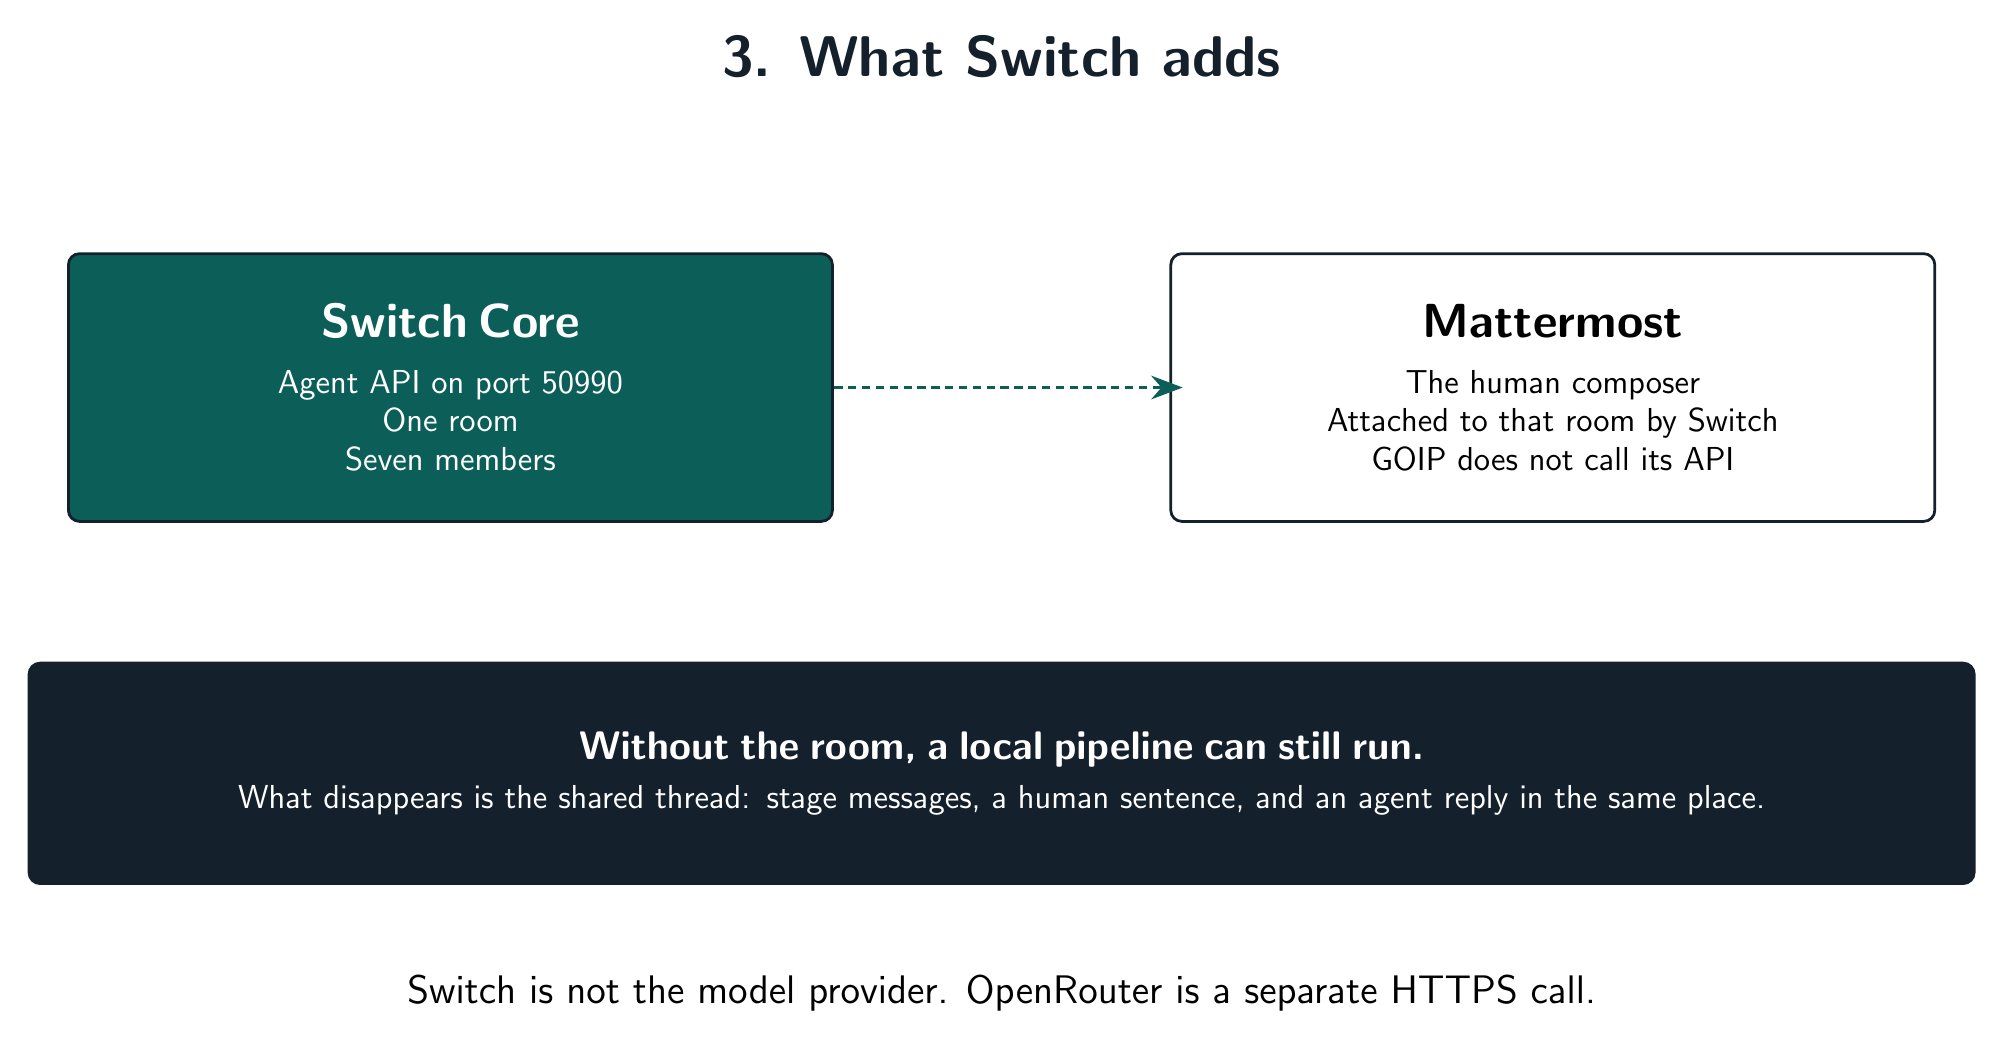
\begin{tikzpicture}
  \node[font=\huge\bfseries, text=ink] at (0,6.5) {3. What Switch adds};
  \node[card, fill=teal, text=white, text width=9cm, minimum height=3.4cm] at (-7,2.3) {{\LARGE\bfseries Switch Core}\\[6pt]\large Agent API on port 50990\\ One room\\ Seven members};
  \node[card, text width=9cm, minimum height=3.4cm] at (7,2.3) {{\LARGE\bfseries Mattermost}\\[6pt]\large The human composer\\ Attached to that room by Switch\\ GOIP does not call its API};
  \node[card, fill=ink, text=white, text width=24cm, minimum height=2.8cm] at (0,-2.6) {{\Large\bfseries Without the room, a local pipeline can still run.}\\[4pt]\large What disappears is the shared thread: stage messages, a human sentence, and an agent reply in the same place.};
  \node[font=\Large, align=center] at (0,-5.4) {Switch is not the model provider. OpenRouter is a separate HTTPS call.};
  \draw[-{Stealth[length=4mm]}, teal, very thick, densely dashed] (-2.3,2.3) -- (2.3,2.3);
\end{tikzpicture}
\end{center}

\newpage
\begin{center}
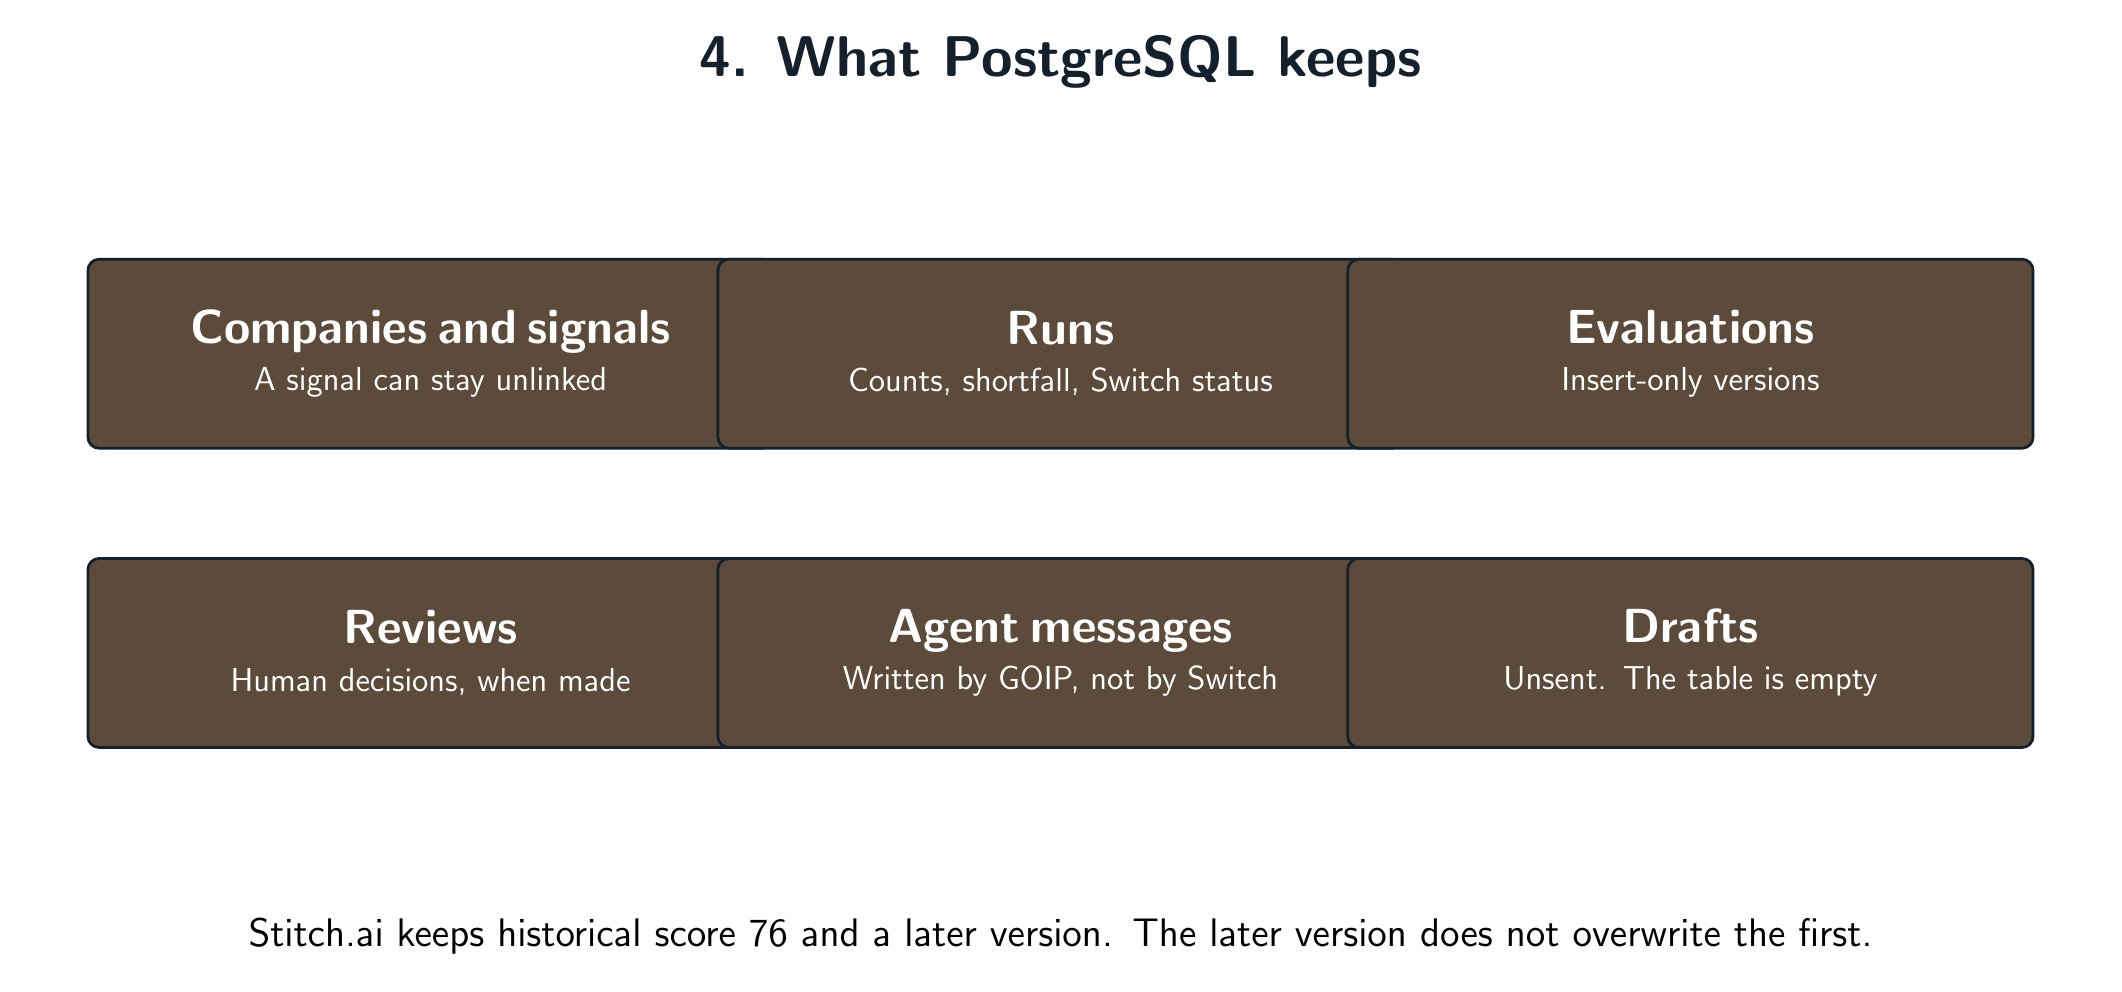
\begin{tikzpicture}
  \node[font=\huge\bfseries, text=ink] at (0,6.5) {4. What PostgreSQL keeps};
  \node[card, fill=brown, text=white, text width=8cm, minimum height=2.4cm] at (-8,2.8) {{\LARGE\bfseries Companies and signals}\\[3pt]\large A signal can stay unlinked};
  \node[card, fill=brown, text=white, text width=8cm, minimum height=2.4cm] at (0,2.8) {{\LARGE\bfseries Runs}\\[3pt]\large Counts, shortfall, Switch status};
  \node[card, fill=brown, text=white, text width=8cm, minimum height=2.4cm] at (8,2.8) {{\LARGE\bfseries Evaluations}\\[3pt]\large Insert-only versions};
  \node[card, fill=brown, text=white, text width=8cm, minimum height=2.4cm] at (-8,-1.0) {{\LARGE\bfseries Reviews}\\[3pt]\large Human decisions, when made};
  \node[card, fill=brown, text=white, text width=8cm, minimum height=2.4cm] at (0,-1.0) {{\LARGE\bfseries Agent messages}\\[3pt]\large Written by GOIP, not by Switch};
  \node[card, fill=brown, text=white, text width=8cm, minimum height=2.4cm] at (8,-1.0) {{\LARGE\bfseries Drafts}\\[3pt]\large Unsent. The table is empty};
  \node[font=\Large, align=center, text width=26cm] at (0,-4.6) {Stitch.ai keeps historical score 76 and a later version. The later version does not overwrite the first.};
\end{tikzpicture}
\end{center}

\newpage
\begin{center}
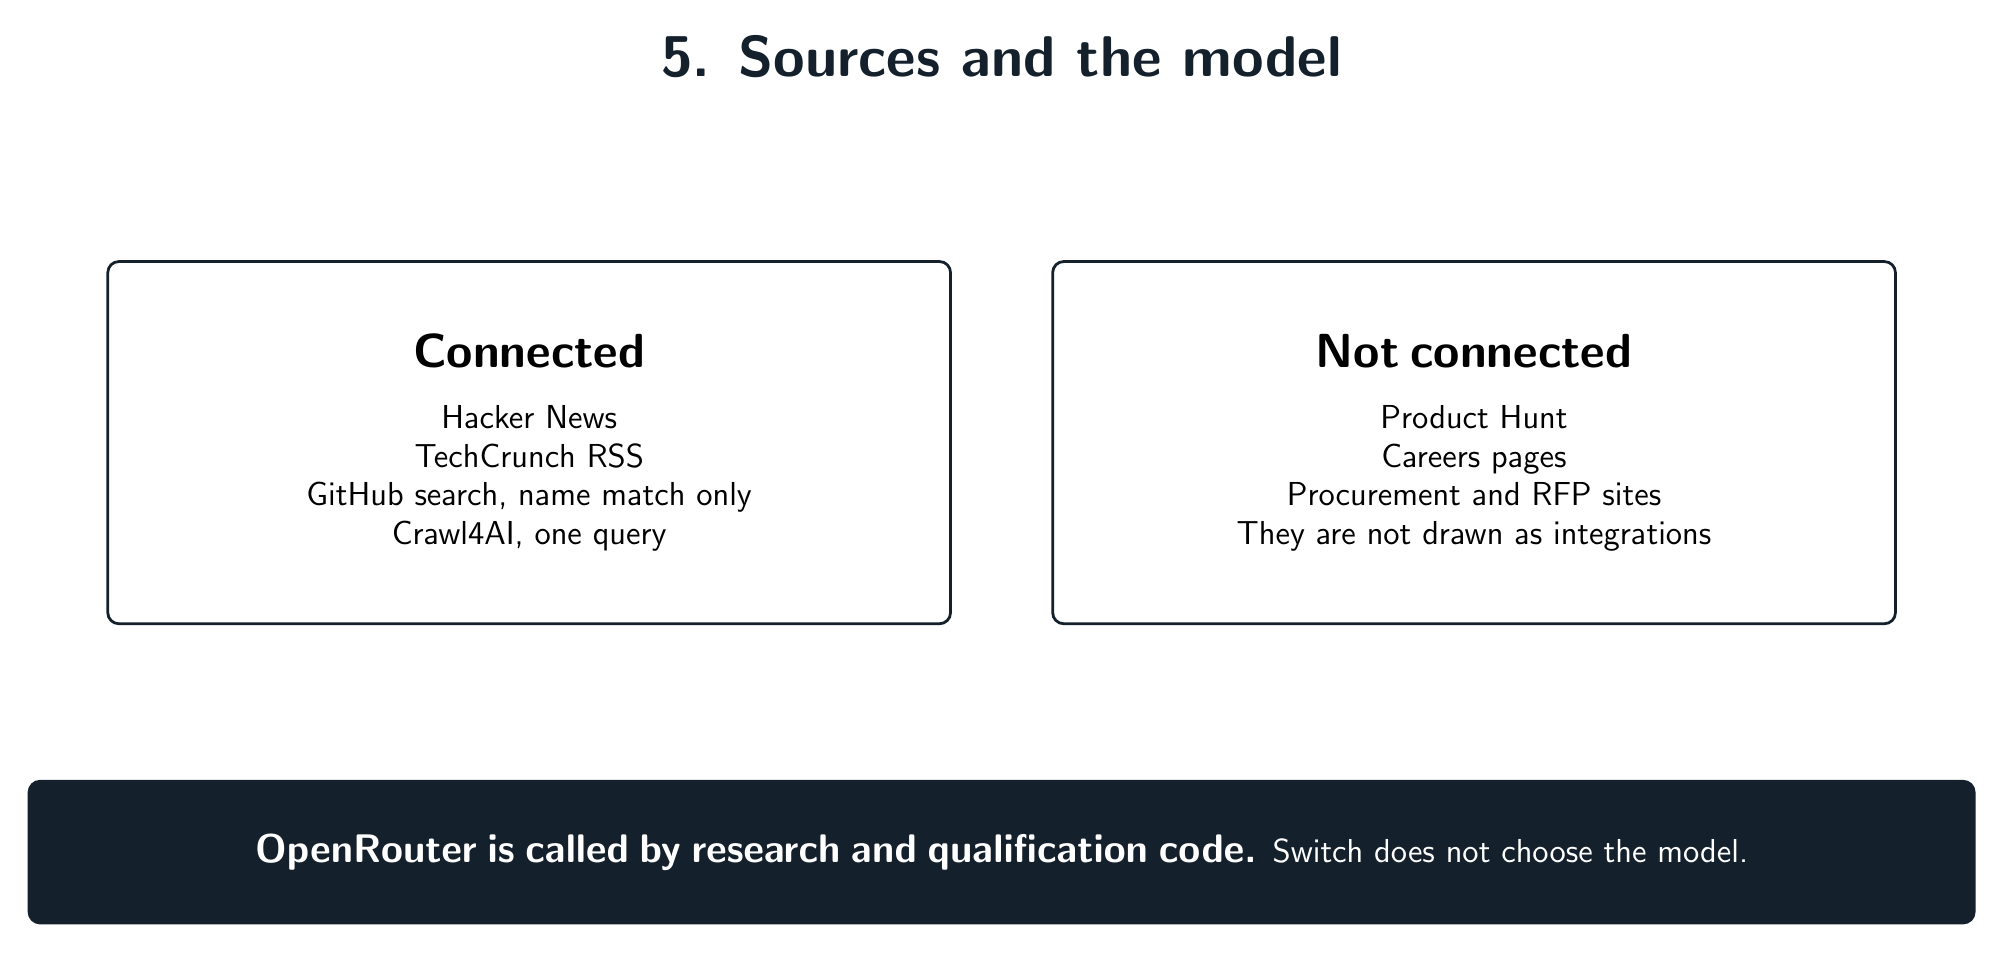
\begin{tikzpicture}
  \node[font=\huge\bfseries, text=ink] at (0,6.5) {5. Sources and the model};
  \node[card, text width=10cm, minimum height=4.6cm] at (-6,1.6) {
    {\LARGE\bfseries Connected}\\[8pt]
    \large Hacker News\\
    TechCrunch RSS\\
    GitHub search, name match only\\
    Crawl4AI, one query
  };
  \node[card, text width=10cm, minimum height=4.6cm] at (6,1.6) {
    {\LARGE\bfseries Not connected}\\[8pt]
    \large Product Hunt\\
    Careers pages\\
    Procurement and RFP sites\\
    They are not drawn as integrations
  };
  \node[card, fill=ink, text=white, text width=24cm, minimum height=1.8cm] at (0,-3.6) {{\Large\bfseries OpenRouter is called by research and qualification code.} Switch does not choose the model.};
\end{tikzpicture}
\end{center}
\end{document}
